%%%%%%%%%%%%
%
% $Autor: Sudeshna,Srikanth,Adhiraj $
% $Datum: 2019-03-05 08:03:15Z $
% $Pfad: Development $
% $Version: 4250 $
% !TeX spellcheck = en_GB/de_DE
% !TeX encoding = utf8
% !TeX root = Development 
% !TeX TXS-program:bibliography = txs:///biber
%
%%%%%%%%%%%%
\section{Data Base}


\section{Data Characteristics}

\begin{enumerate}
	\item \textbf{Structure:}
	
	The JSON structure is organized into \textit{strokes}, each containing an \textit{index} and an array of \textit{stroke points} with X-Y coordinates. This structured format is conducive to representing sequential information, allowing efficient processing and analysis of stroke data.
	
\begin{lstlisting}[language=Python, caption={Example of gesture data with sensor readings}, label={code:gesture-data-json}, style=pythonstyle]
	{
		"gesture_data": [
		{
			"label": "W",
			"sensor_readings": [
			{"acceleration_x": 0.23, "acceleration_y": -0.15, "acceleration_z": 0.98, ...},
			{"acceleration_x": 0.21, "acceleration_y": -0.18, "acceleration_z": 0.95, ...},
			...
			]
		},
		{
			"label": "O",
			"sensor_readings": [
			{"acceleration_x": 0.14, "acceleration_y": 0.22, "acceleration_z": 0.93, ...},
			{"acceleration_x": 0.12, "acceleration_y": 0.20, "acceleration_z": 0.91, ...},
			...
			]
		},
		{
			"label": "L",
			"sensor_readings": [
			{"acceleration_x": -0.10, "acceleration_y": -0.25, "acceleration_z": 0.88, ...},
			{"acceleration_x": -0.12, "acceleration_y": -0.28, "acceleration_z": 0.85, ...},
			...
			]
		},
		...
		]
	}
\end{lstlisting}

	
	
	\item \textbf{Size:}
	
	The dataset comprises a total of 200 labeled instances, providing a robust foundation for training and evaluation. Each gesture type (W, O, L) is well-represented, with over 70 instances for each, ensuring balanced class distribution and supporting reliable model performance.
	
	\item \textbf{Format:}
	
	The dataset is stored in the JSON format, a flexible and widely adopted standard for data representation. Each JSON entry contains a hierarchical structure, including stroke indices, an array of stroke points, and corresponding X-Y coordinates for each point. This structured organization facilitates efficient parsing and analysis, making it ideal for sequential data representation and machine learning applications.
	
	
	\item \textbf{Anomalies:}
	
	Efforts were made to ensure clear and deliberate wand movements during gesture performances to minimize the occurrence of anomalies. A manual review process was applied during the labeling phase to detect and correct any mislabeled or ambiguous instances, thereby enhancing the overall quality and reliability of the dataset.
	
	\item \textbf{Measurement and Screen Size:}
	
	\begin{itemize}
		
		\item \textbf{Accelerometer Measurements:}
		
		Motion data was captured in three dimensions (X, Y, Z) using the accelerometer on the Arduino Nano 33 BLE Sense board. Each gesture was performed within a duration of 1 to 2 seconds, ensuring consistency in the data collection process. The accelerometer's sensitivity enabled precise tracking of gesture dynamics.
		
		\item \textbf{Screen Size:}
		
		A laptop screen with dimensions of 25x30 cm was used for real-time visualization and labeling of recorded gestures. The user interface provided a robust platform for reviewing, labeling, and correcting gesture data, ensuring accurate annotations and facilitating seamless data management.
		
	\end{itemize}
	
	\item \textbf{Origin:}
	
	The dataset for the Magic Wand project originates from the integration of real-world gestures with advanced technology, enabled by the \href{https://tinyml.seas.harvard.edu/magic_wand/}{Magic Wand website}. Our team utilized the Magic Wand Capture sketch, which was uploaded onto the Arduino Nano 33 BLE Sense board, to collect motion data. The user-friendly interface of the website facilitated seamless recording, reviewing, and labeling of unique gestures. This collaborative effort ensured the creation of a diverse and representative dataset, encompassing authentic real-world scenarios and variations among users. The Magic Wand prototype, combined with the Arduino Nano 33 BLE Sense board, served as a crucial tool for capturing nuanced gesture variations. The structured methodology provided by the website significantly contributed to refining the dataset, aligning with the project's objectives and enhancing its utility for practical machine learning applications.
	
\end{enumerate}

The key benefit of expanding a dataset with more input data is that it allows the machine learning model to improve in terms of accuracy, efficiency, and performance. By including additional data, the model can better learn the patterns and characteristics of the gestures. This approach is applied to the remaining gestures, such as ring, slope, and unknown, following the same process. With the data collected for these gestures, we can split the dataset into two parts: one for training the model and another for testing its performance.

A significant challenge in preparing the data is the presence of outliers or anomalies, which are values that deviate significantly from the expected range. These outliers can negatively impact the model's performance. However, one way to address this challenge is by increasing the volume of data to provide a more robust and diverse training set, making the model more resilient to such anomalies. Below are some common types of outliers that may be encountered during data preparation \cite{Munoz:2019}:

\begin{itemize}
	
	\item \textbf{Noise in Accelerometer Readings:}
	
	Environmental interference or external factors during data collection may introduce noise into the accelerometer readings. Outliers can appear as sudden spikes or drops in sensor values that do not correspond to genuine gestures. These are typically considered noise and can be minimized by increasing data points and ensuring proper sensor calibration.
	
	\item \textbf{Abnormal Gesture Patterns:}
	
	Outliers may arise when users perform gestures that deviate from the expected behavior or in an unconventional manner. These abnormal gestures can negatively affect the training process and may distort the model's ability to correctly classify gestures.
	
	\item \textbf{Sensor Malfunctions:}
	
	Outliers can also be a result of sensor malfunctions or inaccuracies in the Arduino Nano 33 BLE Sense device. Issues like sudden jumps, constant offsets, or erratic sensor behavior are typically indicative of hardware problems and should be addressed by either recalibrating the sensors or discarding faulty readings.
	
	\item \textbf{Inconsistent Data Recording:}
	
	Variations in the way users record gestures—such as differences in speed, amplitude, or gesture duration—can lead to inconsistencies in the dataset. It is important to standardize the recording process and eliminate these variations to ensure that the model receives consistent and reliable data for training.
	
	\item \textbf{User-Specific Outliers:}
	
	Each individual may exhibit unique movement patterns or unintentional variations in how they perform gestures. These user-specific outliers can affect the model's ability to generalize across different users. Identifying and addressing these variations, such as normalizing gesture data for different users, is essential for creating a model that works well across a diverse group of individuals.
	
	\item \textbf{Data Transmission Errors:}
	
	Errors or interruptions during the data transmission from the Arduino Nano to the recording system can result in outliers, such as missing or corrupted data points. These transmission errors can be detected and rectified by performing error-checking and data validation techniques during preprocessing to ensure that the dataset is complete and reliable.
	
\end{itemize}

In practice, outliers can be handled in several ways. They can either be removed from the dataset if they are deemed irrelevant or incorrect, or they can be corrected if a reasonable method of rectification is available. Handling outliers effectively ensures that the model can learn from clean, reliable data, improving its accuracy and performance. Additionally, identifying and addressing outliers early in the data preparation process helps create a more robust and generalizable model.

\section{Data Transformation and Data Mining}

The data mining step is the phase where the model is developed and trained to recognize patterns and make predictions. However, before beginning this process, it is crucial to select a suitable algorithm that aligns with the project's objectives and the dataset's characteristics. Factors such as the type of data, computational constraints, and desired output play a key role in this decision. As detailed in the previous section, the dataset is split into training and testing subsets to ensure a fair evaluation of the model’s performance. This division allows for effective testing and validation, enabling the identification of areas for improvement and fine-tuning of the model parameters. Additionally, cross-validation techniques can be employed to enhance reliability and minimize overfitting, ensuring that the model generalizes well to new data \cite{Warden:2020}.

\subsubsection{Training the Model}

To begin our project, we first need to customize one of the example applications included in the SparkFun Edge Board Support Package (BSP) to accommodate the input of our captured dataset. As a prerequisite, follow SparkFun's "Using SparkFun Edge Board with Ambiq Apollo3 SDK" guide to configure the Ambiq SDK and the SparkFun Edge BSP. Once the initial setup is complete, modifications can be made to the example code to handle the dataset appropriately \cite{Laine:2022}.

After adapting the code, the program will be prepared to process the dataset as input. The next step involves building the modified application and flashing it onto the SparkFun Edge device. This ensures the program is ready for testing and data collection.

In the subsequent phase, the three group members will perform the designated motions to construct the dataset. To achieve this, open a terminal window and execute the following command:

\SHELL{script output.txt}

In the terminal interface, connect to the \textcolor{blue}{``115200''} device. Once connected, real-time measurements from the accelerometer will be displayed on the screen. These readings will also be saved in a file named \FILE{output.txt} for further processing. This process ensures an organized and accurate dataset, essential for training and validating the model. Additionally, these steps enable efficient data collection and synchronization, facilitating seamless integration into the project workflow \cite{Warden:2020}.

%\begin{figure}[h!]
%
%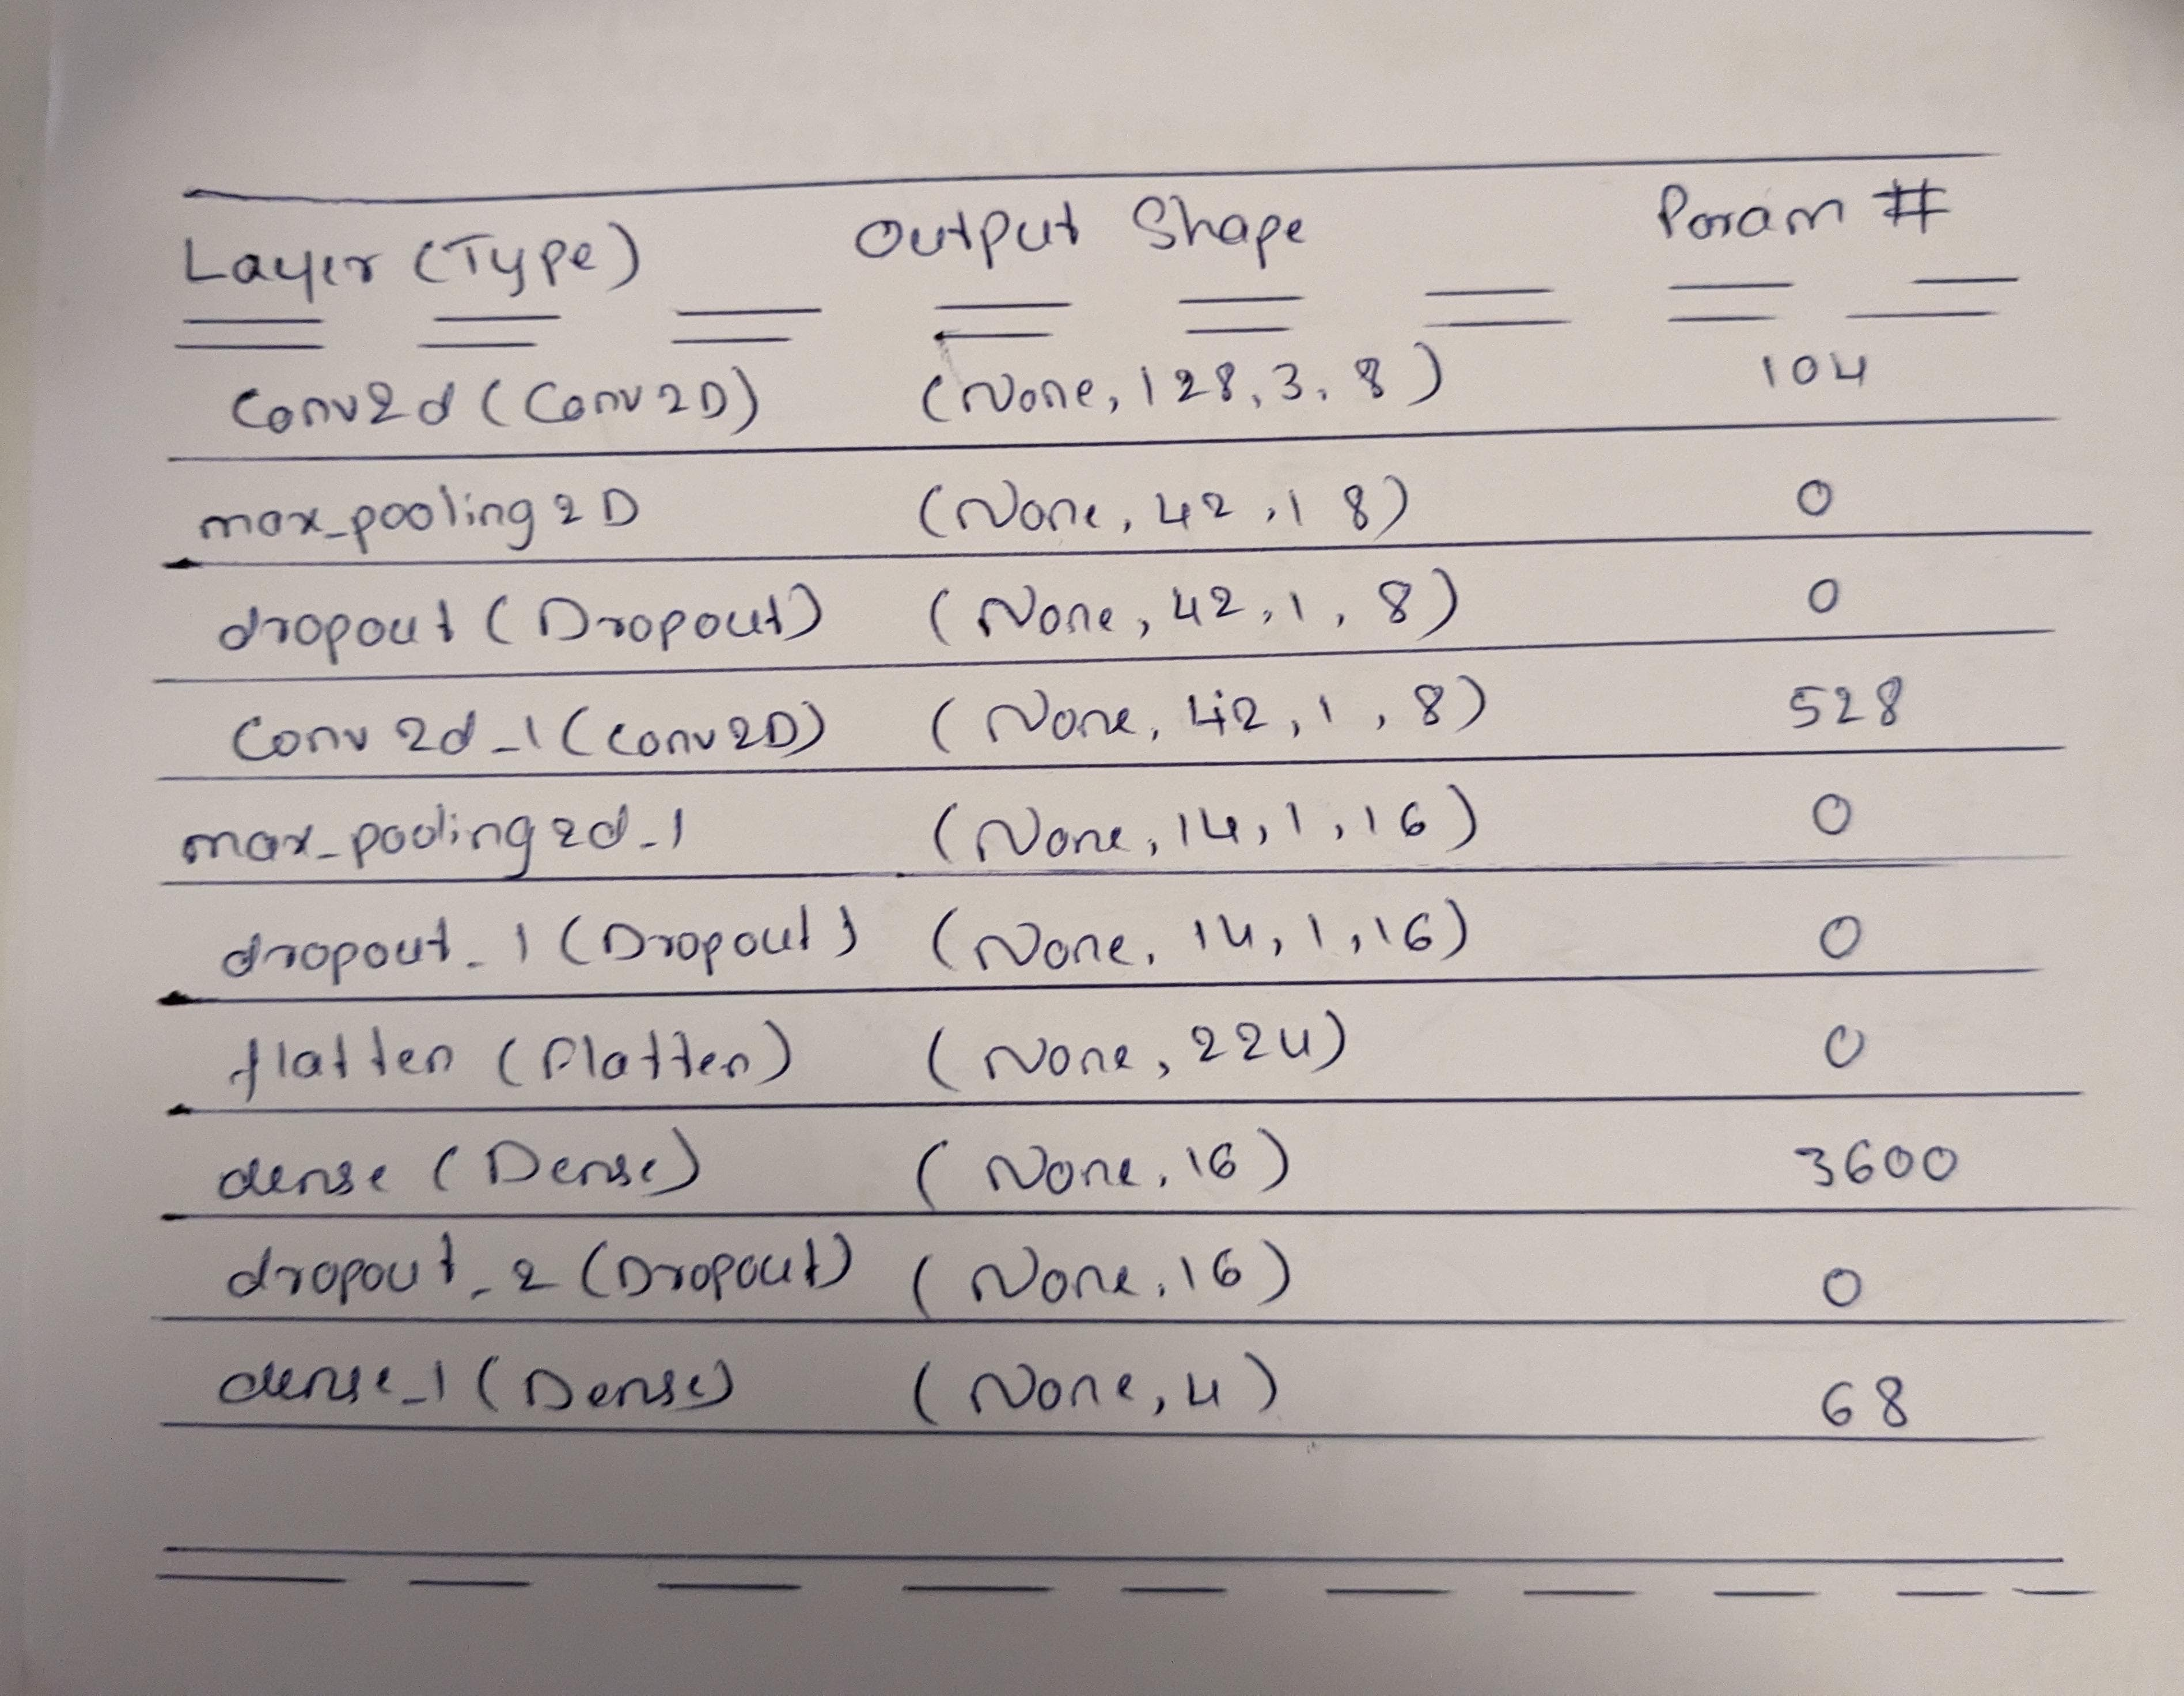
\includegraphics[width=\linewidth]{Images/KDD/Classifygestures}
%\caption{\textbf{\ac{cnn} sequence to classify gestures }}
%\label{Table 7.11}
%
%\end{figure}
\begin{table}
	\caption{\textbf{\ac{cnn} sequence to classify gestures }}
	\label{Table 7.1}
	\begin{center}
		\begin{tabular}{||c c c||} 
			\hline
			Layer (type) & Output Shape & Param\# \\ [0.5ex] 
			\hline\hline
			conv2d(Conv2D) & (None, 128, 3, 8) & 104 \\ 
			\hline
			max\_pooling2d(MaxPooling2D) & (None, 42, 1, 8) & 0 \\
			\hline
			dropout(Dropout) & (None, 42, 1, 8) & 0  \\
			\hline
			conv2d\_1(Conv2D) & (None, 42, 1, 16) & 528 \\
			\hline
			max\_pooling2d\_1(MaxPooling2D) & (None, 42, 1, 16) & 0 \\  
			\hline
			dropout\_1(Dropout) & (None, 42, 1, 16) & 0  \\
			\hline
			flatten(Flatten) & (None, 224) & 0  \\
			\hline
			dense(Dense) & (None, 16) & 3600  \\  
			\hline
			dropout\_2(Dropout) & (None, 16) & 0  \\
			\hline
			dense\_1(Dense) & (None, 4) & 68  \\ [1ex] 
			\hline
		\end{tabular}
	\end{center}
\end{table}	

The text file will store data formatted to meet the training set's requirements. To build a high-quality dataset, each gesture is repeated multiple times to ensure sufficient variation before exiting the program. Once one group member completes this process, the next member records a similar file named \FILE{output.txt}. The logging of accelerometer data can be stopped by pressing the button labeled "14".  

To maintain clarity, the \textcolor{red}{output.txt} files are renamed according to the individuals who performed the gestures. This naming convention helps differentiate datasets and ensures organized testing and validation \cite{Warden:2020}.  

Additionally, data for the "unknown" category is collected and incorporated into the dataset. This step enables the model to classify gestures outside the predefined set as "unknown." With this inclusive data, the training process improves progressively, leading to enhanced validation accuracy over time.  

The following steps are used to train the model:  

\begin{itemize}  
	\item **Loading TensorBoard:** Set up TensorBoard to monitor the training process and visualize metrics.  
	\item **Running Training Code:** Initiate the training process using scripts executed in PyCharm.  
	\item **Data Augmentation:** Execute the \textcolor{red}{data$\_$augmentation} script to enhance the training dataset by introducing variations in acceleration values, providing the model with more diverse input data.  
	\item **Monitoring Output:** Observe the output values displayed on the screen, which include metrics such as the memory size of the model and training progress.  
\end{itemize}  

\subsection{Model}

In this project, the model processes a sequence of 128 three-axis accelerometer readings, corresponding to approximately five seconds of motion, and outputs an array of four probabilities: one for each predefined gesture and one for "unknown." Convolutional Neural Networks (CNNs) are employed due to their ability to capture patterns and relationships within adjacent data points effectively \cite{Warden:2020}. The multi-layered CNN is designed to learn and recognize each gesture by analyzing its fundamental components. For example, it may learn to identify simple up-and-down movements and further understand how combining these with specific z- and y-axis motions forms a "wing" gesture \cite{Warden:2020}.  

A CNN achieves this by employing a series of filters organized in hierarchical layers, where each filter is trained to recognize specific data features. In the initial layer, filters may detect basic structures like an upward acceleration. The identified features are then passed to the next layer, which combines them into more complex structures. For instance, in the "wing" gesture, the "W" shape could be identified by a sequence of four alternating upward and downward accelerations.  

This hierarchical structure enables the CNN to progressively build an understanding of intricate patterns and gestures, resulting in robust and precise classification based on the input accelerometer readings.  

For data acquisition, Inertial Measurement Unit (IMU) signals are utilized \ref{fig:IMU}. The IMU is an electronic component that integrates the accelerometer. The IMU object is derived from the Arduino LSM9DS1 library, which facilitates seamless data collection and processing. This integration ensures efficient and reliable gesture data acquisition, forming the basis for effective training and testing of the CNN model.  

\begin{figure}[h!]
	\begin{center}
		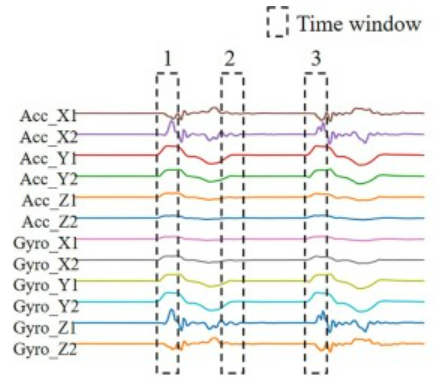
\includegraphics[width=100mm]{Images/KDD/IMU}
		\caption{\textbf{\ac{imu} signals \cite{Xu:2022} }}
		\label{fig:IMU}
	\end{center}
\end{figure}

The convolutional layer is the first component of the network to receive the raw accelerometer data as input. This data is structured into a specific shape, defined by the `input\_shape` argument. The shape is `(seqlength, 3, 1)`, where `seqlength` denotes the total number of accelerometer readings provided, which is 128 by default. Each reading comprises three values corresponding to the x, y, and z axes of motion \cite{Xu:2022}. 

This input format ensures that the network can accurately process the multidimensional nature of the accelerometer data, facilitating the extraction of relevant features for subsequent layers in the model.

\begin{figure}[H]
	\begin{center}
		
		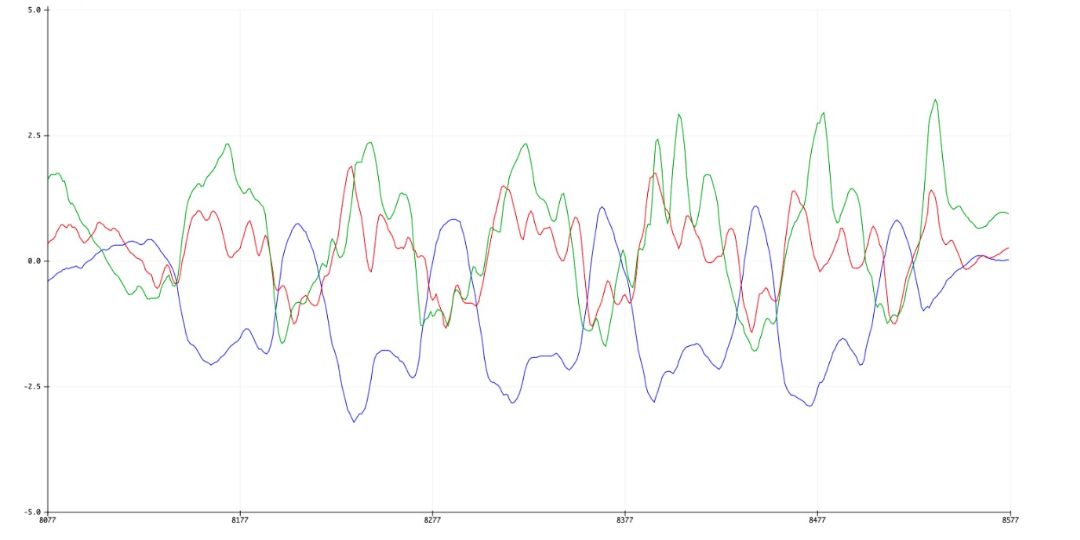
\includegraphics[width=100mm]{Images/KDD/IMUAccelero}
		\caption{\textbf{\ac{imu} Accelerometer Graph}}
		\label{fig:Accel}
		
	\end{center}
\end{figure}

The convolutional layer is responsible for processing raw input data and identifying foundational features that subsequent layers can analyze and interpret. This is achieved through the use of the `Conv2D()` function, which specifies the parameters for feature extraction. The key parameter is the window size, defined in this instance as `(4, 3)`. This configuration implies that the convolutional filter examines four consecutive accelerometer readings across all three axes.

By encompassing four consecutive measurements, each filter effectively captures and analyzes a brief snapshot of time. This allows the model to detect and represent variations in acceleration over time. The process of feature extraction using these filters is visually depicted in \ref{fig:Convolution window}. 

This capability to identify time-dependent changes forms the basis for understanding and classifying gestures, as the extracted features are subsequently passed through the network for further processing and interpretation.

\begin{figure}[H]
	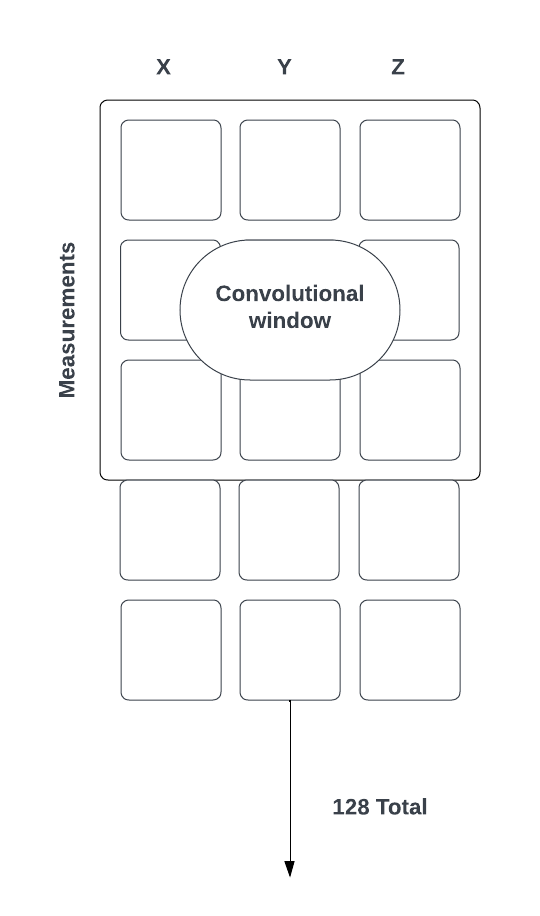
\includegraphics[width=50mm]{Images/KDD/Convolutionwindow}
	\caption{\textbf{A convolution window overlaid on the data}}
	\label{fig:Convolution window}
\end{figure}

The padding argument defines how the filter window moves across the data during convolution operations. When set to "same," the layer's output dimensions remain consistent with the input, maintaining a length of 128 and a width of 3. Each movement of the filter window generates one output value, and with the "same" padding, the window slides across the width three times and down the length 128 times. Once the convolution window completes its traversal, the data is transformed into eight feature maps using the filters. These feature maps are passed to the next layer, MaxPool2D.

The MaxPool2D layer processes the (128, 3, 8) tensor output from the convolutional layer and reduces it to a smaller (42, 1, 8) tensor. This reduction is achieved by sliding a window across the data and selecting the largest value within each window, which is then passed to the output. The size of the sliding window is specified as (3, 3). By default, the window shifts to ensure it processes only new, non-overlapping data. Figure \ref{fig:1212} demonstrates this process \cite{Warden:2020}.

The primary objective of a CNN is to condense a large, intricate input tensor into a smaller, simpler representation. The MaxPool2D layer contributes to this goal by summarizing the first convolutional layer's output into a concentrated, high-level abstraction of the most relevant information. This abstraction helps eliminate irrelevant details, retaining only the most significant features required to identify the gesture.

Following the pooling operation, the data passes through a Dropout layer. Dropout is a regularization method designed to mitigate overfitting by introducing noise. It randomly excludes certain data points between layers, forcing the neural network to adapt to variability and improving its robustness. This layer is active during training but inactive during inference, allowing all data to flow through at that stage \cite{Warden:2020}.

The Dropout layer further refines the input, distilling it into a multidimensional tensor with a shape of (14, 1, 16), representing the critical features of the input data. This process can be repeated by adding more convolutional and pooling layers, with the number of layers acting as a hyperparameter that can be adjusted. In this model, two convolutional layers were deemed sufficient for achieving the desired performance. Figure \ref{fig:CNN sequence} illustrates the CNN's layer sequence.

\begin{figure}[H]
	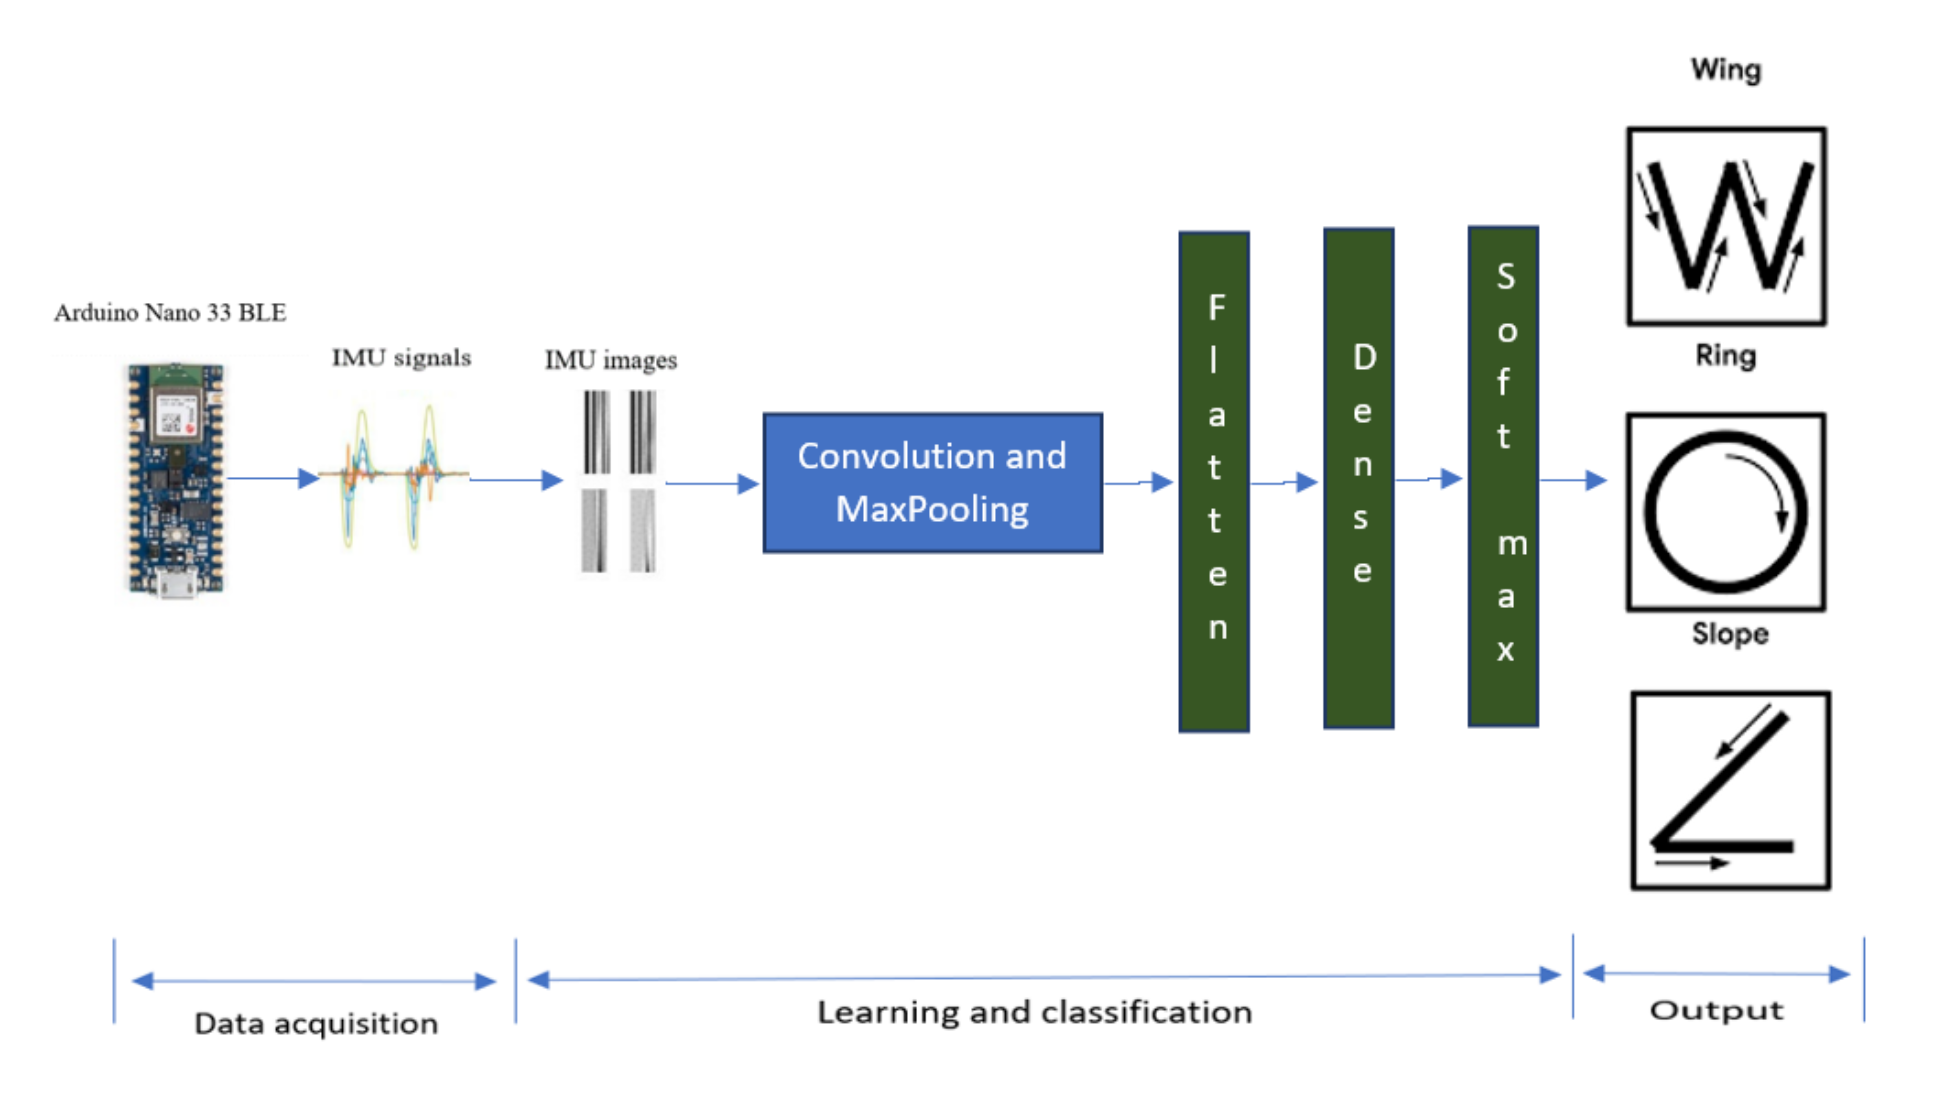
\includegraphics[width=130mm]{Images/KDD/CNNsequence}
	\caption{\textbf{\ac{cnn} sequence to classify Wing,Ring and Slope }}
	\label{fig:CNN sequence}
\end{figure}

We begin by flattening the multidimensional data from the convolutional layers and feeding it into a Dense layer, also called a fully connected layer, to identify the major features in the input. The Flatten layer transforms a tensor with shape \( (14, 1, 16) \) into a one-dimensional tensor with shape \( (224) \). This step condenses the multidimensional data into a single dimension, simplifying further processing.

The resulting flattened tensor is then fed into a Dense layer with 16 neurons. Each neuron in this layer is connected to every input, enabling the model to analyze all features simultaneously and learn the relationships among various combinations of inputs. The Dense layer generates a compressed representation of the input data, summarized into 16 key features \cite{Warden:2020}.

Next, these 16 values are reduced further to represent the four gesture classes: Wing, Ring, Slope, and Unknown. The final Dense layer contains four neurons, each corresponding to one class. These neurons are connected to all 16 outputs from the previous layer. During training, this layer learns the patterns and relationships that identify each gesture class. The layer uses a ``softmax'' activation function, producing output probabilities that sum to 1. This provides a probabilistic classification of the input data into the four classes.

\section*{Gesture Prediction and Validation}
Once the model produces an output tensor containing gesture probabilities, a function called \texttt{PredictGesture()} ensures accurate classification by minimizing false positives. This function performs two key tasks:
\begin{enumerate}
	\item \textbf{Threshold Check}: It verifies that the probability of the detected gesture meets a predefined minimum threshold.
	\item \textbf{Inference Count Check}: It ensures the gesture is consistently detected across a required number of inferences to confirm its validity.
\end{enumerate}

The number of inferences required varies based on the gesture, as each gesture takes a different amount of time to perform. These thresholds and inference requirements are specified in the \texttt{constants.cc} file \cite{Warden:2020}.

The \texttt{PredictGesture()} function returns a numeric value indicating the detected gesture:
\begin{itemize}
	\item \textbf{0}: Wing
	\item \textbf{1}: Ring
	\item \textbf{2}: Slope
\end{itemize}

\section*{Workflow in \texttt{PredictGesture()}}
\begin{enumerate}
	\item The function receives the prediction scores from the main program.
	\item It calculates a \texttt{maxPredictionScore} and identifies the corresponding \texttt{maxPredictionIndex}.
	\item These values are compared with the \texttt{kNoGesture} and \texttt{kDetectionThreshold} constants to determine whether a valid gesture has been identified.
	\item If a gesture is detected, its numeric value (equal to \texttt{maxPredictionIndex}) is assigned to the \texttt{foundGesture} variable.
	\item The \texttt{foundGesture} value is returned to the main function and passed to the \texttt{output\_handler()} function, which displays the recognized gesture.
\end{enumerate}

This combination of convolutional and fully connected layers, paired with a robust validation function, ensures that the model accurately classifies gestures while minimizing false positives. This architecture is particularly effective for analyzing time-series sensor data, such as accelerometer readings, and enables reliable gesture recognition \cite{Warden:2020}.
